\documentclass[oribibl]{llncs/llncs}
\usepackage{color}
\usepackage{graphicx}
\usepackage[caption=false]{subfig}
\usepackage{amsmath}
\allowdisplaybreaks
% \usepackage{amsthm}
\usepackage{amsfonts}
\usepackage{mathtools}
\usepackage{siunitx}
\usepackage[bookmarks]{hyperref}
\usepackage[capitalize]{cleveref}
\usepackage[utf8]{inputenc}
\usepackage{algpseudocode}
\usepackage{algorithm}

\graphicspath{{figures/}}

% Environments
% \newtheorem{theorem}{Theorem}
% \newtheorem{definition}{Definition}
% \newtheorem{problem}{Problem}
% \newtheorem{remark}{Remark}

\crefname{problem}{Problem}{Problems}
\crefname{section}{Sec.}{Secs.}
\crefname{theorem}{Thm.}{Thms.}
\crefname{definition}{Def.}{Defs.}

% Aliases

\newcommand*{\xd}{\dot{x}}
\newcommand*{\R}{\mathbb{R}}
\newcommand*{\N}{\mathbb{N}}

%% Temporal logic symbols
% \newcommand{\not}{\neg}
% \newcommand{\and}{\wedge}
% \newcommand{\or}{\vee}
\newcommand{\Next}{\mathbf{X}}
\newcommand{\Always}{\mathbf{G}}
\newcommand{\Event}{\mathbf{F}}
\newcommand{\luntil}{\mathbf{U}}
\newcommand{\Implies}{\Rightarrow}
\newcommand{\Not}{\lnot}
\newcommand{\True}{\top}

% \newcommand*{\iff}{\Leftrightarrow}

\newcommand*{\psat}[1]{[[#1]]}

\newcommand*{\fran}[1]{\textcolor{blue}{#1}}

\title{Placeholder}

% \author{Francisco Penedo\inst{1} \and Harold S. Park\inst{1} \and Calin Belta\inst{1}}

% \institute{
% Boston University, Boston, MA, U.S.A.\\
% \email{\{franp, parkhs, cbelta\}@bu.edu}
% }

\begin{document}

\maketitle

\begin{abstract}


    In this paper, we introduce a new verification problem with temporal
    specifications for a wide range of linear partial differential equations. 
    We leverage the finite
    element method (FEM) to reduce the problem to a verification problem for
    discrete-time linear systems. The specifications are formalized using a
    novel extension of signal temporal logic (STL) that also admits quantitative
    semantics. A conservative procedure to reformulate the specification into a
    regular STL formula as part of the FEM reduction is also presented. A
    mixed-integer linear encoding is then used to solve the verification problem
    for a set of initial conditions.
    We showcase the conservatism and computational cost of the algorithm on a
    one-dimensional heat equation.

\end{abstract}

\section{Introduction}
\label{sec:introduction}

In the analysis of many engineering problems, it is important to determine
whether, subject to a range of initial and boundary conditions, the system of
interest satisfies certain constraints, or operates within desirable performance
bounds. When the complexity
and diversity of these properties increase, it is useful to state them in
formal languages  that ensure the specification has a
non-ambiguous meaning while being expressive enough to capture many different
behaviors of the system. Among these, temporal logics have enjoyed some
popularity in the fields of robotics, synthetic biology or traffic networks,
besides their original use for digital circuits and computer programs. The
appeal of these formalisms comes from their ability to specify time-related
properties, the availability of verification algorithms, and their resemblance
to natural language.

Many different temporal logics have been proposed tailored to
different kinds of verification problems and systems. Linear Temporal Logic
(LTL) \cite{gerth_simple_1996} and Computational Tree Logic (CTL)
\cite{clarke_automatic_1986} have been widely used to verify
linear- and branching-time properties over infinite time horizons. Probabilistic
versions have been defined and used when verification is considered in a
probabilistic way. For those applications that require explicit time
constraints, such as scheduling or motion planning, we may express properties
using Bounded Linear Temporal Logic (BLTL) \cite{jha_bayesian_2009-1}, Metric
Temporal Logic (MTL) \cite{luo_using_2016}, 
or Time-Window Temporal Logic (TWTL) \cite{AkVaBe-ICRA-2016}. We may additionally be interested in more
than a binary answer to the verification problem, such as how robustly our
system satisfies the specification. In this case, Signal Temporal Logic (STL)
\cite{donze_robust_2010}
admits quantitative semantics that corresponds to the distance of the system
trajectory to the boundary of satisfaction.

In order to formulate a verification problem using a temporal logic, a suitable
model of the system is required. In the case of LTL and CTL, a finite model is
obtained either directly (e.g., for electrical circuits) or through
an abstraction process (e.g., when dealing with dynamical systems described with
differential equations). For the bounded time logics, a full trajectory is
needed, which can present a problem when we attempt to verify the behavior of a
system for a set of initial conditions. One can overcome this issue by using 
a mixed-integer linear encoding of the specification plus the system dynamics in
the case of linear systems \cite{sadraddini_robust_2015}.

The temporal logics discussed so far have only been applied to systems with a
finite-dimensional state space. However, the state space of many interesting systems
is instead a function over some domain, and its time evolution
follows a Partial Differential Equation (PDE). In this work, we extend STL to allow
specifications over the solutions of PDEs and formulate and solve the problem 
of verifying a property in our extension to STL. We consider both verification
with a single initial condition or with a set of initial conditions.
Even though there exists a theory on the often related problem of optimal
control for PDEs (see \cite{lions_optimal_1971}), to the best of our knowledge, the verification 
of temporal properties in systems governed by a PDE has not been explored before.

The approach we take makes use of the Finite Element Method (FEM) to
approximate the trajectory of the PDE by an interpolation of the solution of a
system of Ordinary Differential Equations (ODEs). The FEM is a well-established
numerical method to obtain approximate numerical solutions to PDEs, and is particularly
well-suited to problems with complicated
geometries where exact solutions cannot be found. It works by subdividing, or
discretizing, the domain into small parts (called finite elements), which
imposes an approximation, typically in the form of a low-order polynomial, in
the spatial variation of the field variable of interest. The vertices of the
elements (called the nodes) represent the discrete locations where the unknown
field variables of interest are to be determined; this ocurs through the
assembly of all the unknown nodal degrees of freedom into a global system.
Importantly, the error introduced in moving from a continuous PDE to a discrete
FEM model can be systematically improved by using more elements to discretize
the domain of interest.

In the process of approximating the PDE trajectory by the FEM model and then
discretizing it both in space (considering the finite-dimensional state space
given by the field values at the nodes) and time, we define a conservative
reformulation of the specification that follows the same approximation and
discretization steps. In order to account for the approximation and
discretization errors, the predicates in the formula are perturbed in such a way
that all trajectories satisfying the perturbed predicates also satisfy the
original ones. Finally, we encode the resulting problem into a mixed-integer
linear program (MILP) following previously established methods.

Our method requires the PDE to be linear and also that a FEM approximation to
the PDE can be made. The
latter assumption is not overly restrictive, as the FEM can be applied to all PDEs 
of engineering interest, i.e., Maxwell equations for electromagnetics,
Navier-Stokes equations for fluid dynamics, momentum equation for mechanics,
diffusion and heat equations, and so on. The linear assumption usually constrains the
physical system to linear material behavior, although this assumption is also
not overly restrictive as most engineering systems are designed to operate
within the linear material response regime \cite{}.

\section{Preliminaries}
\label{sec:preliminaries}

\subsection{Finite Element Method}
\label{sec:heat_equation_and_finite_element_analysis}

We provide in this section a brief summary of the Finite Element Method (FEM).
We present the method applied
to a simplified heat equation, although the same technique can be applied to other
PDEs. A more detailed exposition can be found in any
textbook on FEM, such as \cite{hughes_finite_2012-1}.

Let $\Omega = (0, L) \subset \R$ be an open interval representing the interior
of a one-dimensional rod of length $L$; $\rho, c, \kappa > 0$ 
constants denoting density, capacity and conductivity of the rod's material respectively;
$g = (g_0, g_L) \in \R^2$ the boundary conditions at each end of the rod; and $u_0 :
\Omega \rightarrow \R$ an initial value for the temperature on the rod. 
The evolution of the temperature at
each point in the rod can be described by a function $u : \bar \Omega \times [0,
T] \rightarrow \R$, where $T > 0$ denotes the final time and can be infinity and
$\bar \Omega$ is the spatial domain, such that the following initial boundary
value problem (IBVP) is satisfied:

\begin{equation}\label{eq:pde}
    \Sigma^{H}(u_0, g) \quad \left \{
    \begin{aligned}
        \rho c \frac{\partial u}{\partial t} - \kappa \frac{\partial^2
        u}{\partial^2 x} &= 0, \text{on } \Omega \times (0, T) \\
        u(0, t) &= g_0, \forall t \in (0, T) \\
        u(L, t) &= g_L, \forall t \in (0, T) \\
        u(x, 0) &= u_0(x), \forall x \in \Omega
    \end{aligned}
    \right.
\end{equation}

An important aspect of the FEM is the creation of a weak formulation of the
governing PDEs in \cref{eq:pde}. The purpose in deriving a weak form is to
reduce the second order spatial derivative of $u$ in \cref{eq:pde} to first
derivatives so that low order (in this case, linear) polynomials can be used to
approximate the field value $u$. We can construct a weak formulation of \cref{eq:pde} with the same set of
solutions in the following way: let $D$ be the set of sufficiently smooth 
real-valued functions on $\bar{\Omega} \times (0, T)$ such that all 
$u \in D$ satisfies $u(0, t) = g_0, u(L, t) = g_L, \forall t \in (0, T)$, 
and $V$ a similar set of time
independent functions such that all $w \in V$ satisfies $w(0) = w(L) = 0$. 
Find $u \in D$ such that for all $w \in V$,

\begin{equation}\label{eq:weak_pde}
    \begin{aligned}
        &\int_{\Omega} \frac{\partial w}{\partial x} \kappa \frac{\partial
        u}{\partial x} d \Omega + 
        \int_{\Omega} w \rho c \frac{\partial u}{\partial t} d \Omega = 0 \\
        &\int_{\Omega} w \rho c u(\cdot, 0) d \Omega =
        \int_{\Omega} w \rho c u^0 d \Omega \\
    \end{aligned}
\end{equation}

We now obtain an approximate solution to the weak formulation by considering
\cref{eq:weak_pde} with $u$ and $w$ in subspaces of $D$ and $V$.

Let $\{x_i\}_{i = 0}^{n +
1}$, where $x_0 = 0, x_{n+1} = L, x_i \in \Omega, i = 1,...,n$, be a partition of
$\bar\Omega$. Let $d_i(t), i = 0,...,n+1$ represent the
temperature of the rod at node $x_i$, with $d_0(t) = g_0, d_{n+1} = g_L$ and let $d = (d_1, ..., d_n)' \in
\R^n$. We define the following linear node shape function matrices for $i =
0,...,n+1$:

\begin{equation}
    N_i(x) = \begin{cases}
        \frac{x - x_{i - 1}}{x_i - x_{i - 1}} & i > 0, x \in [x_{i-1}, x_i] \\
        \frac{x_{i+1} - x}{x_{i+1} - x_{i}} & i < n+1, x \in [x_{i}, x_{i+1}] 
    \end{cases} 
\end{equation}

which results in the following linear interpolation of the field variable $u$ in
terms of its nodal values $d$:

\begin{equation}
    u^d(x, t) = \sum_{i=0}^{n+1} N_i(x) d_i(t)
\end{equation}

Consider the subspaces $D^h \subset D$ and $V^h \subset V$ of linear
interpolations defined above and time-invariant interpolations respectively.
It can be shown that $u^d(x, t)$ is a solution of the weak formulation over the
sets $D^h$ and $V^h$, where $d$ evolves
according to the following linear system:

\begin{equation}\label{eq:fem}
    \Sigma^H_{FEM}(u_0, g) \quad \left \{
    \begin{aligned}
        \dot{d} &= A d + b(g) \\
        d_i(0) &= u_0(x_i), i = 1,...,n
    \end{aligned}
    \right.
\end{equation}

In the above, $A = -M^{-1}K, b(g) = M^{-1} F(g)$ and $M, K$ and $F$ are the capacity,
stiffness and external force matrices respectively, which are defined as
follows:

% \begin{equation}
    \begin{align}
        M &= \frac{\rho c}{6} \begin{pmatrix}
            2 l_0 + 2 l_1 & l_1  & 0 & \cdots \\ 
            l_1 & 2 l_1 + 2 l_2 & l_2  & \cdots \\ 
            0 & l_2 & 2 l_2 + 2 l_3 &  \cdots \\ 
            \vdots & \ddots & \ddots & \ddots 
        \end{pmatrix} \label{eq:matrices_M} \\
        K &= \kappa \begin{pmatrix}
            \frac{1}{l_0} + \frac{1}{l_1} & -\frac{1}{l_1}  & 0 & \cdots \\ 
            -\frac{1}{l_1} & \frac{1}{l_1} + \frac{1}{l_2} & -\frac{1}{l_2}  & \cdots \\ 
            0 & -\frac{1}{l_2} & \frac{1}{l_2} + \frac{1}{l_3} &  \cdots \\ 
            \vdots & \ddots & \ddots & \ddots 
        \end{pmatrix} \label{eq:matrices_K}\\
        F(g) &= \kappa \begin{pmatrix}
            \frac{g_0}{l_0} \\
            0 \\
            \vdots \\
            0 \\
            \frac{g_L}{l_n}
        \end{pmatrix} \label{eq:matrices_F}
    \end{align}
% \end{equation}

where $l_e = x_{e+1} - x_e$. As a simplifying assumption, we consider the lumped version of $M$, which is
defined as a diagonal matrix resulting from adding all elements in each row of
$M$. Note that with this assumption, $A$ is a banded matrix of bandwidth 3. 
In the following, we will call $\Sigma_{FEM}$ the FEM system corresponding to a
PDE system $\Sigma$.

\subsection{Signal Temporal Logic}
\label{sec:signal_temporal_logic}

% In this section we define a bounded time linear temporal logic suitable to
% formulate specifications for solutions of partial differential equations. We start
% by defining standard Signal Temporal Logic (STL) and then defining a new set of
% predicates over both spatial- and time-varying signals.

In this paper, we base our new specification language for PDEs in Signal
Temporal Logic. An STL formula $\phi$ is defined recursively in the following way:

\begin{equation}
    \phi ::= \mu | \lnot \mu | \phi_1 \land \phi_2 | \phi_1 \luntil_{[a,b]} \phi_2
\end{equation}

where $\mu$ is a predicate over signals of the form $\mu \equiv \mu(s) > 0$,
$\phi_1$ and $\phi_2$ are STL formulas,
$\lnot$ and $\land$ are the Boolean operators negation and conjunction, and
$\luntil_{[a, b]}$ is the bounded temporal operator \emph{until}. The satisfaction
of an STL formula at time $t$ for a signal $s :
\R_{\geq 0} \to \R$ is defined recursively as follows:

\begin{equation}
    \begin{aligned}
        s[t] &\models \mu &\iff &\mu(s(t)) > 0 \\
        s[t] &\models \lnot \mu &\iff &\lnot (s[t] \models \mu) \\
        s[t] &\models \phi_1 \land \phi_2 &\iff &s[t] \models \phi_1 \land s[t]
        \models \phi_2 \\
        s[t] &\models \phi_1 \luntil_{[a,b]} \phi_2 &\iff 
            &\exists t' \in [t+a, t+b] \text{ s.t. } s[t'] \models \phi_2 \\
        & & &\land \forall t'' \in [t, t'] s[t''] \models \phi_1]
    \end{aligned}
\end{equation}

A signal $s$ satisfies an STL formula, $s \models \phi$, if and
only if $s[0] \models \phi$. We define other Boolean operators (disjunction,
implication and equivalence) and constants (true and false) in the usual way, 
and the temporal operators
\emph{eventually} and \emph{globally} as $\Event_{[a, b]} \phi \equiv \top
\luntil_{[a,b]} \phi$ and $\Always_{[a, b]} \phi \equiv \lnot \Event_{[a,b]}
\lnot \phi$ respectively.

We also define quantitative semantics for an STL formula over a signal $s$
using the real valued function $r(\phi, s, t)$, which satisfies the property $s[t]
\models \phi \iff r(\phi,s, t) > 0$ and is computed as follows:

\begin{equation}
    \begin{aligned}
        &r(\mu, s, t) &= &\mu(s(t)) \\
        &r(\lnot \mu, s, t) &= &-r(\mu, s,t) \\
        &r(\phi_1 \land \phi_2, s, t) &= &\min\{r(\phi_1,s, t),
    r(\phi_2,s, t)\} \\
    &r(\phi_1 \luntil_{[a,b]} \phi_2,s, t) &= 
    &\max_{t' \in [t+a, t+b]} \left \{ \min\{ r(\phi_2,s, t), 
\min_{t'' \in [t, t']}\{r(\phi_1,s, t)\}\} \right \}
    \end{aligned}
\end{equation}

We call $r(\phi,s, t)$ the robustness degree of $s$ with respect to $\phi$ at
time $t$.

\section{Signal Temporal Logic for PDEs}
\label{sec:signal_temporal_logic_for_pdes}

In order to define specifications over the trajectories of PDEs, we extend
regular STL using the following set of predicates:
let $\Lambda$ be a set of predicates over
a set $\bar\Omega$, where each predicate $\lambda \in \Lambda$ is defined as a
tuple $(Q_\lambda, X_\lambda, \mu_\lambda)$, 
and represented using the syntax $Q_\lambda x \in X_\lambda : u(x) - \mu_\lambda(x) >
0$, with:

\begin{itemize}
    \item $Q_\lambda \in \{\forall, \exists\}$ is the spatial quantifier,
    \item $X_\lambda \subseteq \bar\Omega$ is the spatial domain of the predicate and
        we require it to be a closed set, and 
    \item $\mu_\lambda : X_\lambda \to \R$ is a continuous and differentiable function 
        representing the reference profile.
\end{itemize}

The set of predicates $\Lambda$ is
said to be compatible with a PDE system $\Sigma$ if $\bar\Omega$ is the spatial
domain of the trajectories of $\Sigma$. We consider STL formulas 
with the previously defined syntax and semantics 
over the set of predicates $\Lambda$, where the satisfaction of a
predicate with respect to a continuous-time signal $u : \bar\Omega \times [0, T]
\to \R$ at time $t \in \R$ is defined as $u[t] \models \lambda \iff 
u(x, t) - \mu_\lambda(x) > 0$ for all $x \in X_\lambda$ if $Q_\lambda = \forall$ or for some $x \in
X_\lambda$ otherwise. We define the quantitative semantics as before with
$r(\lambda,u, t) = \min_{x \in X_\lambda} (u(x, t) - \mu_\lambda(x))$ if $Q_\lambda = \forall$ and
$r(\lambda,u, t) = \max_{x \in X_\lambda} u(x, t) - \mu_\lambda(x))$ otherwise.

\begin{example}
    \label{ex:stl}

    Consider the following formula in STL for a heat equation with a single predicate
    $\lambda = (Q = \forall, X = [8, 9], \mu(x) = -(28x - 192))$, which we 
    represent using the syntax:

    \begin{equation}
        \psi = \Always_{[1,10]} \forall x \in [8,9] : u(x) - (28x - 192) > 0
    \end{equation}

    The specification reads in natural language: ``Always between 1 and 10 time
    units, at all points in a rod between lengths 8 and 9, the temperature
    profile is above the profile $\mu(x) = 28x - 192$."

\end{example}

Throughout this paper, we will use the notation $S(s_0, g) \models \psi$ to denote
that the trajectory of system $S$ (either a PDE system or its corresponding FEM
system) with initial state $s_0$ and boundary conditions $g$ satisfies formula 
$\psi$ (either in regular STL or in STL for PDEs).

\section{Problem Formulation}
\label{sec:problem_formulation}

We can formulate now the STL verification problem for a system governed by a
PDE:

\begin{problem}
\label{pr:stl}
    Given a PDE system $\Sigma$, an STL formula $\psi$ over a set of predicates
    compatible with the system, $\Lambda$, and initial state $u_0$,
    check whether the trajectory of $\Sigma$ for the initial state $u_0$
    satisfies $\psi$.
\end{problem}

A more general problem can be formulated if we consider the initial state to be
in a set:

\begin{problem}
\label{pr:stl_set}
    Given a PDE system $\Sigma$, an STL formula over $\Lambda$, $\psi$, and a set of initial states
    $U_0$, check whether the trajectory of $\Sigma$ satisfies $\psi$ 
    for any initial state $u_0 \in U_0$.
\end{problem}

Finally, we can also formulate a verification problem for PDEs with static
boundary conditions contained in a set. For the sake of clarity, we will not
formulate this problem in its most general form, as the notation required for
the boundary conditions becomes cumbersome.

\begin{problem}
    Given a PDE system $\Sigma$, an STL formula over $\Lambda$, $\psi$, an
    initial state $u_0$, and a set of boundary conditions $G$, check whether the
    system $\Sigma(u_0, g)$ satisfies $\psi$ for any boundary conditions $g \in
    G$.
\end{problem}

Even though the formulation is general for any PDE, in what follows we make two
assumptions on the PDEs that we allow: (1) we can apply FEM to the PDE, and (2)
the system of ODEs obtained is linear. The first assumption imposes no practical
restriction, as FEM is applicable to most PDEs describing physical systems,
including heat conduction, mechanical displacement, fluid mechanics or
mass transportation systems. Assumption (2) on the other hand requires the PDE
to be linear. Additionally, we require in \cref{pr:stl_set} the set of initial
conditions $U_0$ to be described as a polytope in the parameters of a
linear parameterization of the initial conditions. For example, the set $\{u(x)
= a x^2 + b | a \in [1,2], b = 5\}$ is acceptable, while $\{u(x) = a^2 x |
a \in [1,2]\}$ is not.

In order to solve both problems, we first reformulate the specification $\psi$
in such a way that it allows us to solve the verification problems
conservatively on a discrete-time linear system instead. This is done in three
steps by considering the FEM approximation to the real solution, a spatial
discretization and a temporal discretization. The solution of \cref{pr:stl_set}
involves a reformulation into an optimization problem that can be encoded as a
mixed-integer linear program.

\section{Formally Correct Discretization of STL for PDEs}
\label{sec:formally_correct_discretization_of_pdestl}

In this section we define a series of reformulations of an STL formula over
$\Lambda$ such that satisfaction of each successive reformulation guarantees the
satisfaction of the previous one. A diagram showing the hierarchy of the
reformulations is shown in \cref{fig:diagram}. The theory developed in this section is stated
for a general 1D PDE for ease of notation, alghough it applies to higher dimesional PDEs
with minimal changes.

\begin{figure}[!t]
    \centering 
        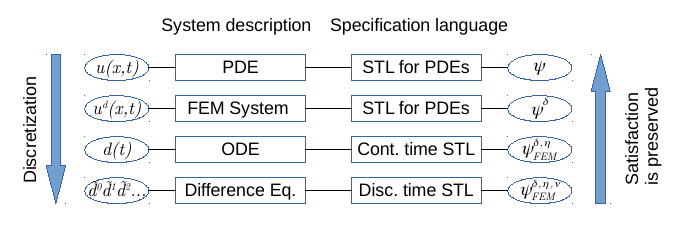
\includegraphics[width=0.99\textwidth]{diagram.png}
    \caption{Summary of our approach to solve the verification problem for a
    PDE.}
    \label{fig:diagram}
\end{figure}


We first reformulate the specification $\psi$ so that we can verify instead the
approximation given by $\Sigma_{FEM}$. Recall that we denote as $u(x,t)$ the
trajectory of $\Sigma$ and $u^d(x, t)$ the piecewise linear approximation
obtained by interpolating the trajectory of $\Sigma_{FEM}$. In the following, we
assume the partition $\{x_i\}_{i=1}^m$ is proposition preserving with respect 
to the set of
regions $\{X_i\}_{i = 1}^{m}$\footnote{This is well defined since the $X_i$ are
closed and there are a finite number of them. In higher dimensions, the
additional requirement that $X_i$ are polytopic is required}. Suppose we are given
an a priori bound, $\epsilon(x, t)$, on the pointwise difference between them, i.e., 
$|u(x, t) - u^d(x, t)| \leq \epsilon(x, t)$.

\begin{definition}
\label{def:m_perturbation}
    Let $\lambda \in \Lambda$ be a predicate
    and let $f : \bar\Omega \to \R$ be a continuous and differentiable function. The perturbation of
    $\lambda$ by $f$, $\lambda^f$, is the predicate given by the tuple
    $(Q_\lambda, X_\lambda,
    \mu^f_\lambda)$, where $\mu^f_\lambda(x, u) = \mu_\lambda(x, u) + f(x)$.
\end{definition}

\begin{definition}
\label{def:delta_perturbation}
    Let $\psi$ be an STL formula over $\Lambda$ in negation normal form 
    and let $\delta : \bar\Omega \to \R$ be a continuous function. The
    conservative perturbation of $\psi$ by $\delta$, $\psi^\delta$, is an STL
    formula in negation normal form obtained by substituting every predicate
    $\lambda$ that appears in $\psi$ in the following way:

    \begin{itemize}
        \item If $\lambda$ is not preceded by a negation operator, then it is
            substituted by $\lambda^{-\delta}$.
        \item Otherwise, it is substituted by $\lambda^{\delta}$
    \end{itemize}

    We will also use $\Lambda^{\delta}$ to refer to the set of all $\delta$ and
    $-\delta$
    perturbations of predicates in $\Lambda$.
\end{definition}

\begin{theorem}
\label{th:epsilon_approximation}
    If $u^d \models \psi^{\delta}$, with $\delta(x) = \max_t \epsilon(x, t)$, then $u \models \psi$.
\end{theorem}
\begin{proof}
    We only need to consider a predicate $\lambda$ and its negation. We have
    \begin{equation}
        \label{eq:th_epsilon}
         |u(x, t) - \mu_\lambda(x) - u^d(x, t) + \mu_\lambda(x)| = 
         |u(x, t) - u^d(x, t)| \leq \delta(x)
    \end{equation}
    Thus, $u(x, t) - \mu_\lambda(x) \geq u^d(x, t) -
    \mu_\lambda(x) - \delta(x)$, which proves the result for $\psi = \lambda$. For $\psi
    = \lnot \lambda$, note that satisfaction is equivalent to $u(x, t) -
    \mu_\lambda(x) < 0$ for $x$ quantified opposite to $Q_\lambda$. Then, from
    \cref{eq:th_epsilon} we have $u(x, t) - \mu_\lambda(x) \leq u^d(x, t) +
    \mu_\lambda(x) - \delta(x)$, completing the proof.
\end{proof}

\begin{example}
    \label{ex:eps_approx}

    Assume we obtain a bound $\delta(x) = 1$ for a heat conduction system
    $\Sigma^H$ with $\Omega = (0, 10)$ and its
    FEM approximation. Consider the same specification $\psi$ defined in \cref{ex:stl}.
    The perturbed specification, $\psi^\delta$ is then:
    
    \begin{equation}
        \psi^\delta = \Always_{[1,10]} \forall x \in [8,9] : u(x) - (28x -
        192) - 1 > 0
    \end{equation}

    If the FEM approximation to $\Sigma^H$ satisfies $\psi^\delta$, we can
    conclude $\Sigma^H$ satisfies $\psi$.
    
\end{example}

\cref{th:epsilon_approximation} gives us a way to conservatively solve
\cref{pr:stl} using the approximation obtained from $\Sigma_{FEM}$.
However, we still need to deal with continuous functions in continuous time. Our
next step will be to reformulate the problem into a verification problem over
the trajectory of $\Sigma_{FEM}$, i.e., $d(t)$.

Let $\Lambda^{\delta}_{FEM} = \{\alpha_{\lambda, e} | \lambda \in
\Lambda^{\delta}, e \in E_{\lambda}\} \cup \{\beta_{\lambda, j} | \lambda \in
\Lambda^{\delta}, j \in J_{\lambda}\}$, where $E_{\lambda} = \{e | [x_e, x_{e+1}] \subseteq
X_{\lambda}\}, J_{\lambda} = \{j | x_j \in X_\lambda, [x_{j-1}, x_j] \not\subseteq
X_\lambda, [x_{j}, x_{j+1}] \not\subseteq X_\lambda \}$,
and satisfaction of $\alpha_{\lambda, e}$ and $\beta_{\lambda, j}$ by 
a continuous-time signal $d : [0, T] \to \R^n$
is defined in the following way:

\begin{equation}
    d[t] \models \alpha_{\lambda, e} \iff y_e(t) - 
    \mu_\lambda(\frac{x_e + x_{e + 1}}{2}) > 0 
\end{equation}
\begin{equation}
     d[t] \models \beta_{\lambda, j} \iff d_j(t) - \mu_\lambda(x_j) > 0
\end{equation}

where $y_e = \frac{d_e(t) + d_{e+1}(t)}{2}$. The robustness degree for these
predicates is defined as in \cref{sec:signal_temporal_logic}.
Note that this set of predicates includes the perturbations defined in
\cref{def:delta_perturbation}. We define perturbations of predicates in
$\Lambda^{\delta}_{FEM}$ by a real number $k$ in a manner analogous to
\cref{def:m_perturbation}, and we denote it as $\alpha^k$.

\begin{definition} 
\label{def:eta_approximation}
    The STL formula over $\Lambda^{\delta}_{FEM}$, $\psi^{\delta, \eta}_{FEM}$, corresponding to an STL
    formula in negation normal form, $\psi^\delta$, over $\Lambda^\delta$, with
    $\eta : \bar\Omega \to \R$, is a formula obtained by substituting every
    predicate $\lambda$ in $\psi^\delta$ by the formula $\bigoplus_{e \in
    E_\lambda} \gamma_{\lambda,e} \oplus \bigoplus_{j \in J_\lambda} \beta_{\lambda, j}$, 
    where $\oplus = \wedge$ if $Q_i = \forall$ and $\oplus = \vee$
    otherwise, and $\gamma_{\lambda,e}$ is defined as the following STL formula:

    \begin{itemize}
        \item If $\lambda$ is not preceded by a negation operator, then
            $\gamma_{\lambda, e} = \alpha_{\lambda, e}^{-k_e}$.
        \item Otherwise, $\gamma_{\lambda, e} = \alpha_{\lambda, e}^{k_e}$.
    \end{itemize}

    In both cases, 

    \begin{equation}
    \begin{aligned}
        k_e = \frac{x_{e+1} - x_e}{2} & \left (\max_{c \in [x_e, x_{e+1}]}
        |\mu'(c)| + \max_{c \in [x_e, x_{e+1}]} \eta(c) \right )
    \end{aligned}
    \end{equation}

    We will abuse the notation and use $\psi^{\delta, 0}_{FEM}$ when referring
    to the formula obtained without perturbing the predicates, i.e., both $\eta$
    and $\mu'$ are considered 0.
\end{definition}
% \frac{\partial u}{\partial x}(c, t)

\begin{theorem}
\label{th:eta_approximation}
    If $d \models \psi^{\delta, \eta}_{FEM}$, with $\eta(x) \geq \max_t |\frac{\partial
    u^d}{\partial x}(x, t)|$, then $u^d \models \psi^\delta$.
\end{theorem}
\begin{proof}
    We only need to consider a predicate $\lambda$ and its negation. We assume
    $Q_\lambda = \forall$, the other case is similar. Let $X_\lambda = [x_a,
    x_b]$. First note that satisfying $\lambda$ is equivalent to satisfying all
    predicates of the set $\{(Q_\lambda, [x_e, x_{e+1}], \mu_\lambda) | e \in
    E_\lambda\}$. For any $e \in E_\lambda$, let $m = \frac{x_e + x_{e+1}}{2}, 
    h = \frac{x_{e+1} - x_{e}}{2}$. 
    For $x \in [x_e, x_{e+1}]$ we have:

    \begin{equation}
    \begin{aligned}
        &|u^d(x, t) - \mu_\lambda(x) - u^d(m, t) + \mu_\lambda(m)| \leq \\
        &h \max_{c \in [x_e, x_{e+1}]} 
        |\mu'(c) + \frac{\partial u^d}{\partial x}(c, t)|
        \leq \\
        &h \left (  
        \max_{c \in [x_e, x_{e+1}]} |\mu'(c)| +
        \max_{c \in [x_e, x_{e+1}]} |\frac{\partial u^d}{\partial x}(c, t)|
        \right ) \leq \\
        &h \left (  
        \max_{c \in [x_e, x_{e+1}]} |\mu'(c)| +
        \max_{c \in [x_e, x_{e+1}]} \eta(c)
        \right )  = K_e
    \end{aligned}
    \end{equation}

    Then, $u^d(x, t) - \mu_\lambda(x) \geq u^d(m, t) - \mu_\lambda(m) - K_e =
    y_e(t) - \mu_\lambda(m) - K_e$, so $d \models \alpha^{-K_e}_{\lambda, e}$
    implies $u^d \models (Q_\lambda, [x_e, x_{e+1}], \mu_\lambda)$ and the
    theorem holds for $\psi^\delta = \lambda$. To prove it for the negated
    predicate, we can follow an argument similar to the one in the proof of
    \cref{th:epsilon_approximation}.
\end{proof}

\begin{example}
    \label{ex:eta_approx}

    Continuing with \cref{ex:eps_approx}, assume we obtained the FEM
    approximation using the partition $\{0.5 i | i \in 0,...,20\}$ and we found the
    bound $\eta(x) = 4$. Note that $|\mu'(x)| = 28$ for all $x$. The perturbed STL
    specification corresponding to $\psi^\delta$ is

    \begin{equation}
        \psi^{\delta, \eta}_{FEM} = \Always_{[1,10]} \bigl(
            (y_{16} - 39 - 1 - k > 0) \land (y_{17} - 53 - 1 - k > 0)
        \bigr)
    \end{equation}

    with $k = \frac{0.5 (28 + 4)}{2} = 8$. If we prove satisfaction of $\psi^{\delta,
    \eta}_{FEM}$ by $\Sigma^H_{FEM}$, we can conclude the interpolation satisfies
    $\psi^\delta$.
    
\end{example}

Finally, we reformulate the problem into a verification problem over the
trajectory of a time discretization of $\Sigma_{FEM}$ with time interval $\Delta
t \in \R$. There are several options at this point: the simplest one is to
consider $\Sigma_{FEM}$ as a first order linear system (augmenting the state
space if needed) and define the time discretization as the following difference
equation:

\begin{equation}
    \label{eq:disc_system}
    \Sigma_{FEM}^{\Delta t}(d(0), g) \quad \left\{
    \begin{aligned}
        \tilde d^{k+1} &= \tilde A \tilde d^k + \tilde b(g) \\
        \tilde d^0 &= d(0)
    \end{aligned}
    \right.
\end{equation}

where $\tilde A = e^{A \Delta t}$ and $\tilde b(g) = - e^{A \Delta t} A^{-1} \left
( e^{- A \Delta t} - I \right ) b(g)$. Note that, in theory, $d(k \Delta t) = \tilde d^k,
\forall k \in \N$. However, in practice one needs to numerically compute the
exponential matrices in $\tilde A$ and $\tilde b$, which introduces an
approximation error difficult to control. As an alternative, we can use any
numerical integration algorithm with fixed time step appropriate to the specific
PDE system under study, several of which have been
thoroughly analyzed in the FEM literature, such as the Newmark family. Similar
to the FEM approximation, assume we have a bound on the approximation error of
the integration algorithm, $\max_k |d_j(k \Delta t) - \tilde d^k_j| \leq
\epsilon^d_j, i=1,2,...$.
% We define satisfaction of an STL formula by a discrete time
% signal in a similar way to continuous time. However, we make a slight abuse of
% notation so that the time bounds for the temporal operators should be understood
% in the continuous sense, i.e, $\tilde d[k] \models \Always_{[a, b]} \psi \iff 
% \forall j \in [\frac{a}{\Delta t}, \frac{b}{\Delta t}] \cap \N, \tilde d^{k + j} \models
% \psi$ and similarly with the eventually operator.

We define a conservative perturbation of $\psi^{\delta, \eta}_{FEM}$ by a real
vector $\nu = (\nu^y, \nu^d)$, $\psi^{\delta, \eta, \nu}_{FEM}$, in a similar
way to \cref{def:eta_approximation}, noting that the predicate $\gamma_{\lambda, e}$ is perturbed
using the constant $l_e^y = \Delta t \nu^y_e$ and the predicate $\beta_{\lambda, j}$ is
perturbed using the constant $l_j^d = \Delta t \nu^d_j$. We abuse the notation
for STL formulas so that we can consider satisfaction of the discrete time
signal $\tilde{d}$. In particular, $\tilde{d}[t] \models \mu \iff
\mu(\tilde{d}^{t / \Delta t}) > 0$.

\begin{theorem}
    \label{th:nu_approximation}
    If $\tilde d \models \psi^{\delta, \eta, \nu}_{FEM}$, with
    $\nu^y_e = \max_t \frac{|\dot d_e(t)| + |\dot d_{e+1}(t)|}{2} +
    \frac{\epsilon^d_e + \epsilon^d_{e+1}}{2}$ and $\nu^d_j = \max_t
    |\dot d_j(t)| + \epsilon^d_j$, then $d \models \psi^{\delta, \eta}_{FEM}$.
\end{theorem}
\begin{proof}
    Similar to \cref{th:eta_approximation}.
\end{proof}

\begin{example}
    \label{ex:nu_approx}

    Continuing with \cref{ex:eta_approx}, assume we discretize $\Sigma_{FEM}$ using
    the timestep $\Delta t = 0.1$ and let $\nu = (5, 5, ...)$. The final
    perturbed specification is

    \begin{equation}
        \psi^{\delta, \eta, \nu}_{FEM} = \Always_{[1,10]} \bigl(
            (y_{16} - 39 - 1 - k - \frac{5}{10} > 0) \land (y_{17} - 53 - 1 - k
            - \frac{5}{10} > 0)
        \bigr)
    \end{equation}

    As before, we can guarantee the satisfaction of $\psi^{\delta,
    \eta}_{FEM}$ by $\Sigma^H_{FEM}$ if $\Sigma_{FEM}^{H, \Delta t}$ satisfies
    $\psi^{\delta, \eta, \nu}_{FEM}$.
    
\end{example}

The main result in this work is a corollary of the previous theorems, which
allows us to solve \cref{pr:stl}
conservatively by solving a verification problem for regular STL and discrete-time
linear systems. 

\begin{theorem}
    If $\Sigma_{FEM}^{\Delta t}(d^0) \models \psi^{\delta, \eta, \nu}_{FEM}$, with $\delta, \eta$
    and $\nu$ defined as in \cref{th:epsilon_approximation,th:eta_approximation,th:nu_approximation}
    and $d^0_i = u_0(x_i), i = 1,...,n$, then $\Sigma(u_0) \models \psi$.
\end{theorem}

We can also obtain a bound on the robustness of the
original specification with respect to the trajectory of $\Sigma$ by making the
following observation:

\begin{theorem}
    \label{th:robustness}
    If $u, u^d, d$ and $\tilde{d}$ are trajectories of $\Sigma$, interpolation
    of $\Sigma_{FEM}$, $\Sigma_{FEM}$ and $\Sigma_{FEM}^{\Delta t}$,
    respectively, and $\psi$ is an STL formula over $\Lambda$, then the 
    following inequality holds:

    \begin{equation}
        r(\psi, u, t) \geq r(\psi^{\delta}, u^d, t) \geq r(\psi^{\delta,
        \eta}_{FEM}, d, t) \geq r(\psi^{\delta, \eta, \nu}_{FEM}, \tilde{d}, t)
    \end{equation}
\end{theorem}
\begin{proof}
    It follows from the proofs of
    \cref{th:epsilon_approximation,th:eta_approximation,th:nu_approximation}.
\end{proof}

\section{Verification of Initial Sets}
\label{sec:verification_of_initial_sets}

In this section we formulate an optimization problem equivalent to
\cref{pr:stl_set} which can be converted to a mixed-integer linear program
(MILP). This program can then be solved using an off-the-shelf solver such 
as Gurobi \cite{gurobi}.

We can reformulate \cref{pr:stl_set} as the following optimization problem:

\begin{equation}
    \label{eq:stl_set_opt}
    \begin{aligned}
        &r_m = &\min \quad &r(\psi^{\delta, \eta, \nu}_{FEM}, \tilde{d}, 0) \\
        &  &\text{s.t. } &\cref{eq:disc_system} \\
        &  & &u^{\tilde{d}}(\cdot, 0) \in U_0
    \end{aligned}
\end{equation}

If $r_m > 0$, then $\psi$ is satisfied for the initial set $U_0$. This
optimization problem is clearly non-convex, due to the $\max$ and $\min$
operators present in the definition of robustness, and the objective function is
non-differentiable. However, we can apply the technique described in
\cite{sadraddini_robust_2015} to
represent robustness as mixed-integer linear constraints. On the other hand, the
system dynamics are linear and we assume the initial set can be represented as
linear constraints over $\tilde{d}^0$. Therefore, \cref{eq:stl_set_opt} is a
MILP.

A solution to \cref{pr:stl_bound_set} can be found with a similar optimization
problem:

\begin{equation}
    \label{eq:stl_bound_set_opt}
    \begin{aligned}
        &r_m = &\min \quad &r(\psi^{\delta, \eta, \nu}_{FEM}, \tilde{d}, 0) \\
        &  &\text{s.t. } &\cref{eq:disc_system} \\
        &  & &u^{\tilde{d}}(\cdot, 0) = u_0 \\
        &  & &g \in G \end{aligned}
\end{equation}

In this case, we need $G$ to be polytopic for the previous optimization problem
to be a MILP. Note that we can combine \cref{eq:stl_set_opt,eq:stl_bound_set_opt} in order to
solve a problem with both sets of initial states and sets of boundary
conditions. In general, we can use \cref{eq:stl_bound_set_opt} with any time-independent 
parameter in the PDE that appears
as an independent term in the FEM system (with respect to other unknowns). We
present an example in \cref{sub:linear_elasticity} for a second order PDE.

The computational time needed to solve a MILP grows exponentially with 
the number of binary variables. In our encoding, we introduce one
binary variable for each argument to a $\min$ or $\max$ function. Thus, the
number of binary variables is proportional to the length of time intervals (in
the discrete sense), the number of boolean connectives in the original formula
$\psi$ and the length of the discretized predicates obtained in
\cref{def:eta_approximation}. In terms of parameters of the problem and solution,
the length of the discrete-time intervals is proportional to the length of the time
intervals in $\psi$ and inversely proportional to $\Delta t$; regarding the
spatial discretization of the predicates, its length is proportional to the size
of the spatial domains and inversely proportional to the size of the partition
(i.e., the distance between two nodes in the partition).

\section{Examples}
\label{sec:examples}

In this section we solve some instances of \cref{pr:stl,pr:stl_set} and discuss
the conservativeness of our approach as well as the computational performance.
We implemented our framework using Python 2.7 and Gurobi 7.0 as our MILP solver.
We ran our implementation in an Intel Core i7 at 2.4GHz and 8GB RAM. In order to
better understand the cost of computing the STL reformulations and building the
MILP model, we performed the robustness computations in single initial state
problems by solving a similar MILP to \cref{eq:stl_set_opt}.

\subsection{Heat Equation}
\label{sub:heat_equation}

We consider first the verification of a single initial value using uniform
meshes of different sizes. Consider a rod with parameters $L = 10, \rho = 1, c =
1, \kappa = 1, g_0 = 10, g_L = 100$, initial value $u_0(x) = 20.0$
for $x \in (0, L)$, $u_0(0) = g_0, u_0(L) = g_L$, and the specification from
\cref{ex:stl}, which we restate here:

\begin{equation}
    \psi = \Always_{[1,10]} \forall x \in [8,9] : u(x) - (28x - 192) > 0
\end{equation}

We show in \cref{fig:ex1_evolution} the trajectory for two mesh sizes along with the
profile in the specification.

\begin{figure}[!t]
    \centering 
    \subfloat[$h = 1.0$]{\label{fig:ex1_a}
        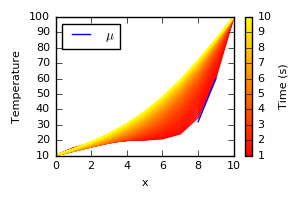
\includegraphics[width=0.49\textwidth]{ex1_plots10.png}}
        \hfill
    \subfloat[$ h = 0.2$]{\label{fig:ex1_b}
        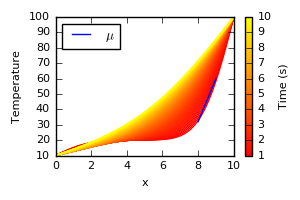
\includegraphics[width=0.49\textwidth]{ex1_plots50.png}}
        \hfill
    \caption{Trajectory $u^d(x, t)$ for two mesh sizes and the reference
        temperature profile $\mu(x) = 28x - 192$. Note how the trajectory
        obtained with a coarser mesh satisfies the specification, while the one
        obtained with a finer mesh does not.}
    \label{fig:ex1_evolution}
\end{figure}


Throughout this
section we will consider the true trajectory of the system for some initial
value, $u^*(x, t)$, the solution of the associated FEM system with a uniform mesh of
size $h = 0.01$. We also set $\Delta t = 0.1$ for all time discretizations.

We computed the bound $\delta(x) = \delta$ as the maximum pointwise
error between simulations of the true trajectory and the trajectory for the
given mesh using random initial values of the form $u_0(x) = \min\{\max\{a x +
b, g_0\}, g_L\}$ with $|a| < 2 |g_L - g_0| / L$ and $b \in (0, |g_L - g_0|)$.
Likewise, we determined the bounds $\eta(x)$ and $\nu$ from those simulated
trajectories. We show in \cref{fig:bounds} the resulting bounds for two mesh
sizes.

\begin{figure}[!t]
    \centering 
    \subfloat[$h = 0.5$]{\label{fig:bounds_a}
        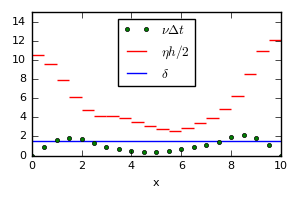
\includegraphics[width=0.49\textwidth]{pert_plot_N20.png}}
        \hfill
    \subfloat[$ h = 0.2$]{\label{fig:bounds_b}
        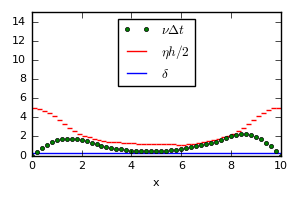
\includegraphics[width=0.49\textwidth]{pert_plot_N50.png}}
        \hfill
    \caption{Bounds used for $\delta$, $\eta$ and $\nu$ multiplied by their
    respective coefficients in the perturbation terms. Note that we show $\nu^d_j$ at
    $x_j$ and use $\nu_e^y = \frac{\nu^d_j + \nu^d_{j+1}}{2}$}
    \label{fig:bounds}
\end{figure}

The robustness results are shown in \cref{tab:res_meshes}. As expected, finer meshes
yield robustness values closer to the true robustness.

\begin{table}
\centering
\begin{tabular}{|c|c|c|c|c|c|c|}
    \hline
    $h$ & $\delta$ & $r(\psi_{FEM}^{0, 0, 0})$ & $r(\psi_{FEM}^{\delta, 0, 0})$ &
    $r(\psi_{FEM}^{\delta, \eta, 0})$ & $r(\psi_{FEM}^{\delta, \eta,
\nu})$ & Time (s)  \\
    \hline
    1 & 5.29 & 1.66 & -3.44 & -32.25 & -34.10 & 0.5 \\
    0.5 & 1.49 & -1.57 & -2.93 & -18.61 & -20.61 & 1.5 \\
    0.33 & 0.68 & -2.29 & -2.92 & -13.34 & -15.47 & 3.6 \\
    0.25 & 0.37 & -2.68 & -3.03 & -10.55 & -12.72 & 5.9 \\
    0.2 & 0.24 & -2.74 & -2.94 & -9.10 & -11.27 & 9.9 \\
    \hline
\end{tabular}
\caption{Verification of a single initial value. Robustness of the true
trajectory is -2.7}
\label{tab:res_meshes}
\end{table}

We checked the validity of our approach as well as the degree of
conservativeness that the perturbations add by verifying random initial values
of the previous form. We used for this example a uniform mesh of size $h = 0.2$
and the following specification: 

\begin{equation}
    \begin{aligned}
        \phi &= \Always_{[1, 10]} \forall x \in [1, 9]: u(x) - 9x > 0 \\
        &\wedge \Event_{[4, 6]} \lnot \exists x \in [6, 7]: u(x) - (9x + 15) > 0
\end{aligned}
\end{equation}

which reads in natural language: ``Always between 1 and 10 time units, at all
points in the rod between lengths 1 and 9, the temperature profile is above the
profile $\mu_1(x) = 9x$. Additionally, eventually between 4 and 6 time units,
there does not exist a point in the rod between lengths 6 and 7 such that the
temperature profile is above the profile $\mu_2(x) = 9x + 15$." We depict the
profiles in the specification in \cref{fig:ex2_evolution}, along with two
trajectories.

\begin{figure}[!t]
    \centering 
    \subfloat[$a = 8.5, b = 10.0$]{\label{fig:ex2_a}
        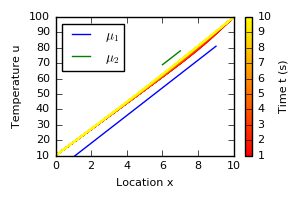
\includegraphics[width=0.49\textwidth]{ex2_plots0.png}}
        \hfill
    \subfloat[$a = 5.0, b = 20.0 $]{\label{fig:ex2_b}
        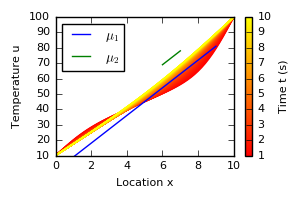
\includegraphics[width=0.49\textwidth]{ex2_plots1.png}}
        \hfill
        \caption{Two sample trajectories of $u^d(x, t)$ using a mesh of size
        $h=0.2$ and the reference profiles $\mu_1 = 9x$ and $\mu_2 = 9x + 15$}
    \label{fig:ex2_evolution}
\end{figure}


We show in \cref{fig:res_diffs} the difference between the true robustness and
the robustness for our mesh, both with and without the perturbations. Note that
when we include all perturbations, the computed robustness is less than the true
robustness, hence we correctly verify as satisfying all examples
that are satisfying. Regarding the conservatism of the approach, we obtain a
difference of at most 5.5 degrees in the robustness, which would allow us to verify a
specification that is satisfied by at least 5.5 degrees at all points in a system
that ranges through 90 degrees. It took an average of 19.29 seconds with a
standard deviation of 1.00 to verify the perturbed formula.

\begin{figure}
    \centering
    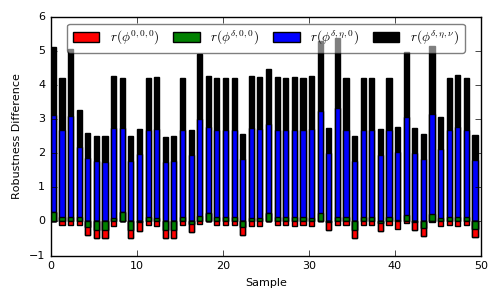
\includegraphics[width=0.8\linewidth]{figures/cs_ran_init_results.png}
    \caption{Difference between true robustness and robustness of the
        discretized specification with and without perturbations for
        random initial values}
    \label{fig:res_diffs}
\end{figure}


Finally, we verified the specification for sets of initial conditions of the
form $u_0(x) = a x + b$ with $a$ and $b$ constrained as before. Again we use a
mesh of size $h = 0.2$. We summarize our results in \cref{tab:res_sets}. We
marked as undefined satisfaction the cases in which the minimum robustness is
negative, since we cannot guarantee their non-satisfaction.

\begin{table}
\centering
\begin{tabular}{|c|c|c|c|c|}
    \hline
    $a$ & $b$ & Minimum robustness & Result & Time (s)  \\
    \hline
    9 & [5, 13] & 0.5 & Satisfies & 21 \\
    9 & [5, 15] & -0.7 & Undefined & 22 \\
    9 & [0, 10] & -2.8 & Undefined & 22 \\
    $[8, 10]$ & [5, 13] & -5.0 & Undefined & 379 \\
    $[8.5, 9.5]$ & [8, 10] & 0.5 & Satisfies & 326 \\
    $[5, 12]$ & [0, 20] & -29.6 & Undefined & 82 \\
    \hline
\end{tabular}
\caption{Verification of sets of initial values}
\label{tab:res_sets}
\end{table}

\subsection{Linear Elasticity}
\label{sub:linear_elasticity}

Consider a steel rod of length $L = \SI{100}{}$, density $\rho = \SI{7.24e-4}{}$ and Young's
modulus $E = \SI{30e6}{}$ with one end fixed and a force $h_L$ applied to the
other end. The displacement $u(x, t)$ of the rod follows the following IBVP:

\begin{equation}\label{eq:pde_mech}
    \Sigma^{M}(u_0, v_0, h_L) \quad \left \{
    \begin{aligned}
        \rho \frac{\partial^2 u}{\partial^2 t} - E \frac{\partial^2
        u}{\partial^2 x} &= 0, \text{on } \Omega \times (0, T) \\
        u(0, t) &= 0, \forall t \in (0, T) \\
        \rho \frac{\partial^2 u}{\partial^2 t}(L, t) &= h_L, \forall t \in (0, T) \\
        % u(L, t) &= g_L, \forall t \in (0, T) \\
        u(x, 0) &= u_0(x), \forall x \in \Omega \\
        \frac{\partial u}{\partial t}(x, 0) &= v_0(x), \forall x \in \Omega
    \end{aligned}
    \right.
\end{equation}

where $u_0, v_0$ are the initial displacements and velocities.
The corresponding FEM system for linear elements is given by:

\begin{equation}\label{eq:fem_mech}
    \Sigma^M_{FEM}(u_0, v_0, h_L) \quad \left \{
    \begin{aligned}
        M\ddot{d} + K d &= F + F_{nodal}(h_L) \\
        d_i(0) &= u_0(x_i), i = 1,...,n \\
        \dot{d}_i(0) &= v_0(x_i), i = 1,...,n
    \end{aligned}
    \right.
\end{equation}

where $F_{nodal}(h_L) = (0, 0, ..., 0, h_L)^T$ is the nodal force vector, and $M, K, F$ 
are the mass, stiffness and force matrices, respectively, and
they have the same expressions as in
\cref{eq:matrices_M,eq:matrices_K,eq:matrices_F}, with $c = 1, \kappa = E$.
For this example, we use the central differences algorithm to obtain a time
discretization with time interval $\Delta t$. The resulting difference equations
are the following:

\begin{equation}
    \Sigma^{M, \Delta t}_{FEM}(d^0, v^0, h_L) \quad \left \{
    \begin{aligned}
        \tilde v^{n+1} &= v^n + \frac{1}{2} \Delta t a^n \\
        \tilde d^{n+1} &= \tilde d^{n} + \Delta t \tilde v^{n+1} \\
        M a^{n+1} &= F + F_{nodal}(h_L) - K \tilde d^{n+1} \\
        v^{n+1} &= \tilde v^{n+1} + \frac{1}{2} \Delta t a^{n+1} \\
        M a^0 &= F + F_{nodal}(h_L) - K d^0 \\
    \end{aligned}
    \right.
\end{equation}

A classical engineering problem related to the safety of this system is to
verify that the maximum displacements at all points in the rod do not exceed a
safe profile. We formulate an STL specification that captures the behavior in
the following way:

\begin{equation}
    \phi_1 = \Always_{[0.001, 0.005]} \lnot \exists x \in [20, 80]: u(x) - 7 \cdot
    10^{-5} x - 10^{-3} > 0
\end{equation}

We solve the verification problem assuming the rod starts at rest ($u_0 = 0,
v_0 = 0$) and the foce $h_L$ is contained in the set $[900, 1100]$.

We also consider a more complicated specification that refers to the periodic
behavior of the system:

\begin{equation}
\begin{aligned}
    \phi_2 &= \Always_{[0.001, 0.005]} \bigl( \Event_{[0, 0.002]} \forall x \in [20,
    80]: u(x) - 3 \cdot 10^{-5} x > 0 \\
    &\land \Event_{[0, 0.002]} \lnot \exists x
    \in [20, 80]: u(x) - (7 \cdot 10^{-5}x - 0.5 \cdot 10^{-3}) > 0\bigr)
\end{aligned}
\end{equation}

which reads in natural language: ``For \SI{0.004}{\second} since
\SI{0.001}{\second}, within intervals of \SI{0.002}{\second} the displacements
at every point between lengths \SI{20}{} and \SI{80}{} are above the profile
$\mu_1(x) = 3 \cdot 10^{-5} x$ and below the profile $\mu_2(x) = 7 \cdot 10^{-5} x
- 0.5 \cdot 10^{-3}$."

\section{Conclusion}
\label{sec:conclusion}

In this paper, we formulated and solved a verification problem for systems governed by a
PDE with specifications given in a novel extension to STL. Our solution relies
on the approximation of the PDE using the Finite Element Method, which reduces
the problem to the verification of a standard STL formula for a discrete-time
linear system. The reformulation requires perturbing the predicates in the
formula using the FEM approximation errors as well as the derivatives of the
approximated solution and the predicate functions. Finally, the final
verification problem is encoded as a MILP.

We implemented our method in Python and used Gurobi to solve the MILP. Our
results on a simple heat equation show an acceptable level of conservatism that
would allow us to verify a specification satisfied more robustly than a 6\% of the range of
the system. We were able to solve verification problems for sets of initial conditions in a
few minutes on consumer hardware.

As future work, we want to find the bounds $\delta, \eta$ and $\nu$ in a
systematic way, either analytically or using a robust statistical method. We
also plan to formulate and solve control problems for PDEs under STL constraints
using a similar approach.

\bibliographystyle{llncs/splncs03}
\bibliography{bibliography}


\end{document}
